\documentclass[12pt,utf8,notheorems,compress,t]{beamer}
\usepackage{etex}

\usepackage{pgfpages}
\setbeameroption{show notes on second screen}
\setbeamertemplate{note page}[plain]
\newcommand{\jnote}[2]{\only<#1>{\note{\setlength\parskip{\medskipamount}\justifying\footnotesize#2\par}}}

% Workaround for the issue described at
% https://tex.stackexchange.com/questions/164406/beamer-using-href-in-notes.
\newcommand{\fixedhref}[2]{\makebox[0pt][l]{\hspace*{\paperwidth}\href{#1}{#2}}\href{#1}{#2}}

\usepackage[english]{babel}

\usepackage{mathtools}
\usepackage{booktabs}
\usepackage{stmaryrd}
\usepackage{array}
\usepackage{ragged2e}
\usepackage{multicol}
\usepackage{tabto}
\usepackage{xstring}
\usepackage{ifthen}
\usepackage[normalem]{ulem}
\usepackage[all]{xy}
\xyoption{rotate}
\usepackage{tikz}
\usetikzlibrary{calc,shapes,shapes.callouts,shapes.arrows,patterns,fit,backgrounds,decorations.pathmorphing}
\hypersetup{colorlinks=true}

\usepackage{pifont}
\newcommand{\cmark}{\ding{51}}
\newcommand{\xmark}{\ding{55}}
\DeclareSymbolFont{extraup}{U}{zavm}{m}{n}
\DeclareMathSymbol{\varheart}{\mathalpha}{extraup}{86}

\graphicspath{{images/}}

\usepackage[protrusion=true,expansion=true]{microtype}

\setlength\parskip{\medskipamount}
\setlength\parindent{0pt}

\title{A general Nullstellensatz for generalized spaces}
\author{Ingo Blechschmidt}
\date{April 11st, 2019}

\useinnertheme[shadow=true]{rounded}
\setbeamerfont{block title}{size={}}

\useinnertheme{rectangles}

\usecolortheme{orchid}
\usecolortheme{seahorse}
\definecolor{mypurple}{RGB}{150,0,255}
\setbeamercolor{structure}{fg=mypurple}
\definecolor{myred}{RGB}{150,0,0}
\setbeamercolor*{title}{bg=myred,fg=white}
\setbeamercolor*{titlelike}{bg=myred,fg=white}
\setbeamercolor{frame}{bg=black}

\usefonttheme{serif}
\usepackage[T1]{fontenc}
\usepackage{libertine}

% lifted from https://arxiv.org/abs/1506.08870
\DeclareFontFamily{U}{min}{}
\DeclareFontShape{U}{min}{m}{n}{<-> udmj30}{}
\newcommand\yon{\!\text{\usefont{U}{min}{m}{n}\symbol{'210}}\!}

\newcommand{\A}{\mathcal{A}}
\newcommand{\B}{\mathcal{B}}
\renewcommand{\C}{\mathcal{C}}
\newcommand{\M}{\mathcal{M}}
\renewcommand{\AA}{\mathbb{A}}
\newcommand{\E}{\mathcal{E}}
\newcommand{\F}{\mathcal{F}}
\renewcommand{\G}{\mathcal{G}}
\newcommand{\J}{\mathcal{J}}
\newcommand{\GG}{\mathbb{G}}
\renewcommand{\O}{\mathcal{O}}
\newcommand{\K}{\mathcal{K}}
\newcommand{\NN}{\mathbb{N}}
\newcommand{\QQ}{\mathbb{Q}}
\newcommand{\RR}{\mathbb{R}}
\newcommand{\TT}{\mathbb{T}}
\newcommand{\PP}{\mathbb{P}}
\newcommand{\ZZ}{\mathbb{Z}}
\newcommand{\CC}{\mathbb{C}}
\renewcommand{\P}{\mathcal{P}}
\newcommand{\aaa}{\mathfrak{a}}
\newcommand{\ppp}{\mathfrak{p}}
\newcommand{\fff}{\mathfrak{f}}
\newcommand{\defeq}{\vcentcolon=}
\newcommand{\defeqv}{\vcentcolon\equiv}
\newcommand{\Sh}{\mathrm{Sh}}
\newcommand{\GL}{\mathrm{GL}}
\newcommand{\Zar}{\mathrm{Zar}}
\newcommand{\op}{\mathrm{op}}
\newcommand{\Set}{\mathrm{Set}}
\newcommand{\Eff}{\mathrm{Ef{}f}}
\newcommand{\Sch}{\mathrm{Sch}}
\newcommand{\Aff}{\mathrm{Aff}}
\newcommand{\Ring}{\mathrm{Ring}}
\newcommand{\LocRing}{\mathrm{LocRing}}
\newcommand{\LRS}{\mathrm{LRS}}
\newcommand{\Hom}{\mathrm{Hom}}
\newcommand{\Spec}{\mathrm{Spec}}
\newcommand{\lra}{\longrightarrow}
\newcommand{\RelSpec}{\operatorname{Spec}}
\renewcommand{\_}{\mathpunct{.}}
\newcommand{\?}{\,{:}\,}
\newcommand{\speak}[1]{\ulcorner\text{\textnormal{#1}}\urcorner}
\newcommand{\ul}[1]{\underline{#1}}
\newcommand{\affl}{\ensuremath{{\ull{\AA}^1}}}
\newcommand{\Ll}{\vcentcolon\!\Longleftrightarrow}
\newcommand{\inv}{inv.\@}
\newcommand{\seq}[1]{\mathrel{\vdash\!\!\!_{#1}}}
\newcommand{\hg}{\mathbin{:}}  % homogeneous coordinates

\setbeamertemplate{blocks}[rounded][shadow=false]

\newenvironment{indentblock}{%
  \list{}{\leftmargin\leftmargin}%
  \item\relax
}{%
  \endlist
}

% Adapted from https://latex.org/forum/viewtopic.php?t=2251 (Stefan Kottwitz)
\newenvironment<>{hilblock}{
  \begin{center}
    \begin{minipage}{9.05cm}
      \setlength{\textwidth}{9.05cm}
      \begin{actionenv}#1
        \def\insertblocktitle{}
        \par
        \usebeamertemplate{block begin}}{
        \par
        \usebeamertemplate{block end}
      \end{actionenv}
    \end{minipage}
  \end{center}}

\newcommand{\bignumber}[1]{
  \renewcommand{\insertenumlabel}{#1}\scalebox{1.5}{\usebeamertemplate{enumerate item}}
}
\newcommand{\bigheart}{
\includegraphics{heart}}

\newenvironment{changemargin}[2]{%
  \begin{list}{}{%
    \setlength{\topsep}{0pt}%
    \setlength{\leftmargin}{#1}%
    \setlength{\rightmargin}{#2}%
    \setlength{\listparindent}{\parindent}%
    \setlength{\itemindent}{\parindent}%
    \setlength{\parsep}{\parskip}%
  }%
  \item[]}{\end{list}}

\tikzset{
  invisible/.style={opacity=0,text opacity=0},
  visible on/.style={alt={#1{}{invisible}}},
  alt/.code args={<#1>#2#3}{%
    \alt<#1>{\pgfkeysalso{#2}}{\pgfkeysalso{#3}}}
}

\newcommand{\pointthis}[3]{%
  \tikz[remember picture,baseline]{
    \node[anchor=base,inner sep=0,outer sep=0] (#2) {#2};
    \node[visible on=#1,overlay,rectangle callout,rounded corners,callout relative pointer={(0.3cm,0.5cm)},fill=blue!20] at ($(#2.north)+(-0.1cm,-1.1cm)$) {#3};
  }%
}

\tikzset{
  invisible/.style={opacity=0,text opacity=0},
  visible on/.style={alt={#1{}{invisible}}},
  alt/.code args={<#1>#2#3}{%
    \alt<#1>{\pgfkeysalso{#2}}{\pgfkeysalso{#3}}}
}

\newcommand{\hcancel}[5]{%
  \tikz[baseline=(tocancel.base)]{
    \node[inner sep=0pt,outer sep=0pt] (tocancel) {#1};
    \draw[red, line width=0.4mm] ($(tocancel.south west)+(#2,#3)$) -- ($(tocancel.north east)+(#4,#5)$);
  }%
}

\newcommand{\explain}[7]{%
  \tikz[remember picture,baseline]{
    \node[anchor=base,inner sep=2pt,outer sep=0,fill=#3,rounded corners] (label) {#1};
    \node[anchor=north,visible on=<#2>,overlay,rectangle callout,rounded corners,callout
    relative pointer={(0.0cm,0.5cm)+(0.0cm,#6)},fill=#3] at ($(label.south)+(0,-0.3cm)+(#4,#5)$) {#7};
  }%
}

\newcommand{\squiggly}[1]{\textcolor{red}{#1}}  % XXX

% Adapted from https://latex.org/forum/viewtopic.php?t=2251 (Stefan Kottwitz)
\newenvironment<>{varblock}[2]{\begin{varblockextra}{#1}{#2}{}}{\end{varblockextra}}
\newenvironment<>{varblockextra}[3]{
  \begin{center}
    \begin{minipage}{#1}
      \begin{actionenv}#4
        {\centering \hil{#2}\par}
	\def\insertblocktitle{}%\centering #2}
        \def\varblockextraend{#3}
	\usebeamertemplate{block begin}}{
        \par
        \usebeamertemplate{block end}
        \varblockextraend
      \end{actionenv}
    \end{minipage}
  \end{center}}

\setbeamertemplate{headline}{%
  \begin{beamercolorbox}[wd=\paperwidth,ht=2.25ex]{}%
    \insertsectionnavigationhorizontal{\paperwidth}{}{}%
  \end{beamercolorbox}%
  \vskip0pt%
}

\setbeamertemplate{frametitle}{%
  \vskip0.6em%
  \leavevmode%
  \begin{beamercolorbox}[dp=1ex,center]{}%
  %   \usebeamercolor[fg]{item}{\textbf{{\Large \insertframetitle}}}
    \begin{tikzpicture}
      \def\R{8pt}
      \node (title) {\hil{\insertframetitle}};
      \begin{pgfonlayer}{background}
      \draw[decoration={bumps,segment length=8pt}, decorate, very thick, draw=mypurple]
        ($(title.south west) + (\R, 0)$) arc(270:180:\R) --
        ($(title.north west) + (0, -\R)$) arc(180:90:\R) --
        ($(title.north east) + (-\R, 0)$) arc(90:0:\R) --
        ($(title.south east) + (0, \R)$) arc(0:-90:\R) --
        cycle;
      \end{pgfonlayer}
    \end{tikzpicture}
  \end{beamercolorbox}%
  \vskip-0.6em%
}

\setbeamertemplate{navigation symbols}{}

\newcounter{framenumberpreappendix}
\newcommand{\backupstart}{
  \setcounter{framenumberpreappendix}{\value{framenumber}}
}
\newcommand{\backupend}{
  \addtocounter{framenumberpreappendix}{-\value{framenumber}}
  \addtocounter{framenumber}{\value{framenumberpreappendix}} 
}

\newcommand{\mynav}[3]{%
  foo
}

\newcommand{\insertframeextra}{}
\setbeamertemplate{footline}{%
  \begin{beamercolorbox}[wd=\paperwidth,ht=2.25ex,dp=1ex,right,rightskip=1mm,leftskip=1mm]{}%
    % \inserttitle
    \hfill
    \insertframenumber\insertframeextra\,/\,\inserttotalframenumber
  \end{beamercolorbox}%
  \vskip0pt%
}


\newcommand{\hil}[1]{{\usebeamercolor[fg]{item}{\textbf{#1}}}}
\newcommand{\bad}[1]{\textcolor{red!90}{\textnormal{#1}}}

\begin{document}

\addtocounter{framenumber}{-1}

%\setbeamertemplate{headline}{\mynav{gray}{gray}{gray}}

{\usebackgroundtemplate{\begin{minipage}{\paperwidth}\vspace*{4.95cm}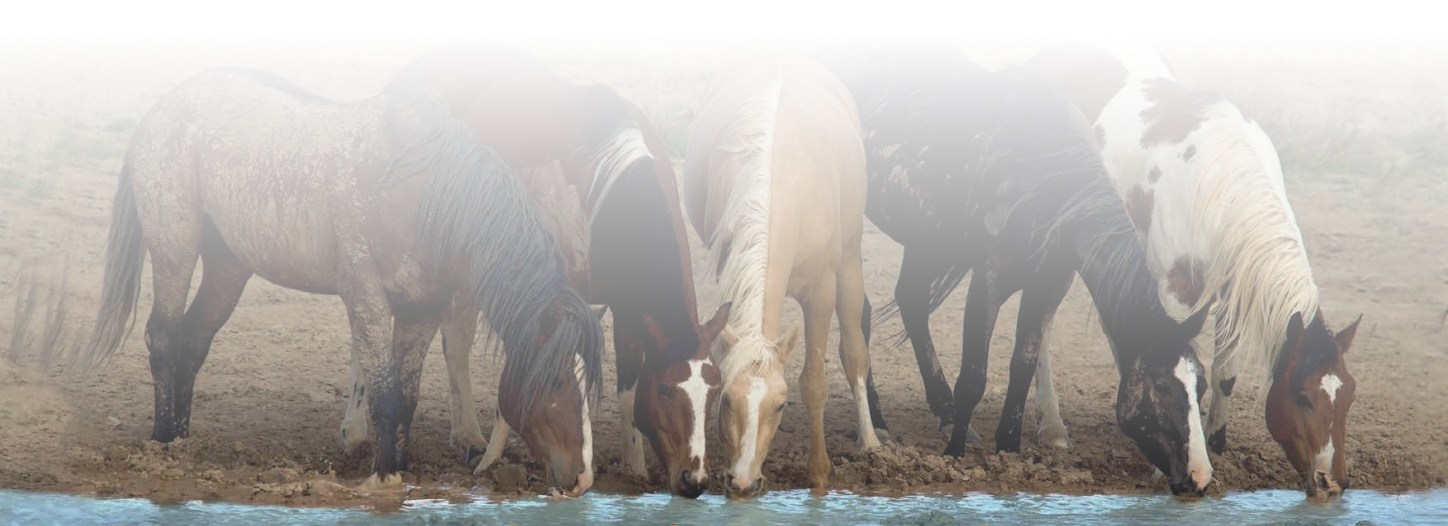
\includegraphics[width=\paperwidth]{topos-horses}\end{minipage}}
\begin{frame}[c]
  \centering

  \bigskip
  
\includegraphics[width=0.4\textwidth]{phantoms}
  \bigskip

  \begin{tikzpicture}
    \def\R{8pt}
    \node (title) {\hil{\ A general Nullstellensatz for generalized spaces\ }};
    \begin{pgfonlayer}{background}
    \draw[decoration={bumps,segment length=8pt}, decorate, very thick, draw=mypurple]
      ($(title.south west) + (\R, 0)$) arc(270:180:\R) --
      ($(title.north west) + (0, -\R)$) arc(180:90:\R) --
      ($(title.north east) + (-\R, 0)$) arc(90:0:\R) --
      ($(title.south east) + (0, \R)$) arc(0:-90:\R) --
      cycle;
    \end{pgfonlayer}
  \end{tikzpicture}

  \scriptsize
  \textit{-- an invitation --}
  \bigskip

  Ingo Blechschmidt \\
  Università di Verona
  \bigskip

  6th Workshop on Formal Topology in Birmingham \\
  April 11st, 2019
  \par
\end{frame}}


\section{The generic model}

\subsection{The mystery of nongeometric sequents}

\begin{frame}{The mystery of nongeometric sequents}
  Let~$\TT$ be a \explain{geometric theory}{4-}{red!20}{-1cm}{0cm}{0cm}{\begin{minipage}{4.3cm}
  sorts,
  function symbols,
  relation symbols,
  geometric sequents as axioms
  \end{minipage}}, for instance the
  \explain{theory of rings}{4-}{blue!20}{-1cm}{0cm}{0cm}{\begin{minipage}{4.3cm}
    \begin{tabbing}
      fun. symb.: \= \kill
      sorts: \> $R$ \\
      fun. symb.: \> $0$, $1$, $-$, $+$, $\cdot$ \\
      % rel. symb.: \> \emph{none} \\
      axioms: \> $(\top \vdash_{x,y:R} x y = y x)$, \ldots
    \end{tabbing}
  \end{minipage}}.

  % Illustration
  \vspace{2.5cm}

  \pause

  \justifying
  \textbf{Theorem.} There is a \hil{generic model}~$U_\TT$. It is
  \hil{conservative} in that
  for any \explain{geometric sequent}{4-}{yellow!70}{0cm}{0cm}{0cm}{
    a sequent of the form~$(\varphi \vdash_{x_1,\ldots,x_n} \psi)$
    where~$\varphi$ and~$\psi$ are geometric formulas
  }~$\sigma$ the following notions coincide:
  \vspace*{-1.2em}
  \begin{enumerate}
    \item The sequent~$\sigma$ holds for~$U_\TT$.
    \item The sequent~$\sigma$ holds for any~$\TT$-model in any
    \explain{topos}{4-}{purple!20}{0cm}{0cm}{0cm}{foo}.
    \item The sequent~$\sigma$ is provable modulo~$\TT$.
  \end{enumerate}

  \pause

  \justifying
  %\textbf{Main observation.} The generic model can validate nongeometric
  %sequents which are not provable modulo~$\TT$ and which do not hold for
  %arbitrary models in arbitrary toposes.

  \textbf{Observation (Kock).} The generic local ring is a field:
  \[ (x = 0 \Rightarrow \bot) \vdash_{x:R} (\exists y\?R\_ xy = 1) \]
\end{frame}


\subsection{Construction of the generic model}

\begin{frame}{Construction of the generic model}
  The generic model is \hil{not} the same as \ldots
  \begin{itemize}
    \item the \hil{initial model}, think~$\ZZ$, or
    \item the \hil{free model on one generator}, think~$\ZZ[X]$.
  \end{itemize}
  Set-theoretic models are \hil{too inflexible}.

  \textbf{Definition.} The \hil{syntactic site}~$\C_\TT$ has \ldots
  \begin{enumerate}
    \item objects: $\{ x_1\?X_1, \ldots, x_n\?X_n\_ \varphi \}$ (shorter:
    $\{ \vec x\_ \varphi \}$)
    \item morphisms: eqv. classes of \explain{provably functional
    formulas}{2-}{red!20}{-2.5cm}{-1.5cm}{0cm}{$\Hom(\{\vec x\_ \varphi\},\{\vec
    y\_ \psi\}) = \{ \theta \,|\, (\theta \seq{\vec x, \vec y} \varphi
    \wedge \psi), (\varphi \seq{\vec x} \exists! \vec
    y\_ \theta) \text{ mod~$\TT$} \}/({\dashv\vdash})$}
    \item coverings: provably jointly surjective families
  \end{enumerate}
  The topos of sheaves over~$\C_\TT$ is the \hil{classifying
  topos}~$\Set[\TT]$. The generic model interprets a sort~$X$ by~$\yon\{x\?X\_\top\}$.
\end{frame}


\subsection{Going internal}

\begin{frame}{Going internal}
  \small
  Let~$\C$ be a site. We recursively define
  \[
    U \models \varphi \quad
    \text{(``$\varphi$ holds on~$U$'')}
  \]
  for objects~$U \in \C$ and \squiggly{formulas}~$\varphi$.
  Write~``$\Sh(\C) \models \varphi$'' to mean~$1_\CC \models \varphi$.
  \footnotesize
  \[ \renewcommand{\arraystretch}{1.08}\begin{array}{@{}l@{\ \ }c@{\ \ }l@{}}
  U \models \top &\Ll& \text{true} \\
  U \models \bot &\Ll& \hcancel{\text{false}}{0pt}{3pt}{0pt}{-2pt}\ \text{the
  empty family is a covering of~$U$} \\
  U \models s = t \? F &\Ll& s|_U = t|_U \in F(U) \\
  U \models \varphi \wedge \psi &\Ll&
  \text{$U \models \varphi$ and $U \models \psi$} \\
  U \models \varphi \vee \psi &\Ll&
  \hcancel{\text{$U \models \varphi$ or $U \models
  \psi$}}{0pt}{3pt}{0pt}{-2pt}\ \text{there exists a covering $(U_i \to U)_i$} \\
  && \quad\quad\text{such that for all~$i$: $U_i \models \varphi$ or $U_i \models \psi$} \\
  U \models \varphi \Rightarrow \psi &\Ll&
  \text{for all~$V \to U$: }
  \text{$V \models \varphi$ implies $V \models \psi$} \\
  U \models \forall s \? F\_ \varphi(s) &\Ll&
  \text{for all $V \to U$ and sections~$s_0 \in F(V)$: $V \models \varphi(s_0)$} \\
  % U \models \forall F\_ \varphi(F) &\Ll&
  % \text{for all $V \to U$ and sheaves~$F_0$ over~$V$: $V \models \varphi(F_0)$} \\
  U \models \exists s \? F\_ \varphi(s) &\Ll&
  \hcancel{\text{there exists $s_0 \in F(U)$ such that $U \models \varphi(s_0)$}}{0pt}{3pt}{0pt}{-2pt} \\
  &&
  \text{there exists a covering $(U_i \to U)_i$ such that for all~$i$:} \\
  && \quad\quad \text{there exists~$s_0 \in F(U_i)$ such that $U_i \models \varphi(s_0)$}
  %U \models \exists F\_ \varphi(F) &\Ll&
  %\hcancel{\text{there exists a sheaf $F_0$ on $U$ such that $U \models
  %\varphi(F_0)$}}{0pt}{3pt}{0pt}{-2pt} \\
  %&&
  %\text{there exists a covering $(U_i \to U)_i$ such that for all~$i$:} \\
  %&& \quad\quad \text{there exists a sheaf~$F_0$ on $U_i$ such that $U_i \models \varphi(F_0)$}
  \end{array} \]
\end{frame}


% \begin{document}

\section{Examples for nongeometric properties}

\begin{frame}{Examples for nongeometric properties}
  The \hil{generic object} validates [XXX]:
  \begin{enumerate}
    \item $\forall x,y\?U_\TT\_ \neg\neg(x = y)$.
    \item $\forall x_1,\ldots,x_n\?U_\TT\_ \neg \forall y\?U_\TT\_
    \bigvee_{i=1}^n y = x_i.$
  \end{enumerate}

  The \hil{generic ring} validates:
  \begin{enumerate}
    \item $\forall x\?U_\TT\_ \neg\neg(x = 0)$.
    \item $\forall x\?U_\TT\_ (x = 0 \Rightarrow 1 = 0) \Rightarrow (\exists
    y\?U_\TT\_ xy = 1)$.
  \end{enumerate}

  The \hil{generic local ring} validates:
  \begin{enumerate}
    \item $\neg \forall x\?U_\TT\_ \neg\neg(x = 0)$.
    \item $\forall a_0,\ldots,a_{n-1}\?U_\TT\_ \neg\neg \exists x\?U_\TT\_
      x^n + a_{n-1}x^{n-1} + \cdots + a_0 x^0 = 0$.
    \item \justifying Let~$\Delta = \{ \varepsilon \? U_\TT \,|\, \varepsilon^2 = 0 \}$.
    For any map~$f : \Delta \to U_\TT$, there are unique elements~$a,b \?
    U_\TT$ such that~$f(\varepsilon) = a + b\varepsilon$ for all~$\varepsilon
    \? \Delta$.
%   \item For any finitely presented~$U_\TT$-algebra~$A$,
%   the canonical map~$A \to (U_\TT)^{\Hom_{U_\TT}(A,U_\TT)}$
%   is an isomorphism.
  \end{enumerate}
\end{frame}


\section{Motivation for generic models}

\begin{frame}{Motivation for generic models}
  Let~$A$ be a ring. Is there a \hil{free local ring}~$A \to A'$ over~$A$?
  \begin{columns}[t]
    \begin{column}{0.4\textwidth}
      $\xymatrix{
        A \ar[rd] \ar[rrr]^\alpha &&& {\substack{\phantom{\text{local}}\\\text{\normalsize$R$}\\\text{local}}} \\
        & {\substack{\text{\normalsize$A'$}\\\text{local}}} \ar@{-->}_[@!35]{\text{local}}[rru]
      }$
    \end{column}

    \begin{column}{0.50\textwidth}
      \small\justifying
      For a fixed ring~$R$, the localization $A' \defeq A[S^{-1}]$ with $S \defeq
      \alpha^{-1}[R^\times]$ would do the job. ($S$ is a \emph{filter}.)
      \medskip

      Hence we need the \hil{generic filter}.
    \end{column}
  \end{columns}

  \pause

  \justifying
  The free local ring over~$A$ is~$A^\sim \defeq \underline{A}[F^{-1}]$,
  where~$F$ is the generic filter, living in~$\Spec(A)$, the classifying topos
  of filters of~$A$.

  \pause

  If~$A$ is reduced ($x^n = 0 \Rightarrow x = 0$):

  \vspace*{-0.8em}
  \setbeamercolor{block body}{bg=red!30}
  \setbeamercolor{structure}{fg=purple}
  \begin{varblock}{\textwidth}{}
    $A^\sim$ is a \hil{field}: $\forall x\?A^\sim\_ (\neg(\exists y\?A^\sim\_
    xy = 1) \Rightarrow x = 0)$.

    $A^\sim$ has \hil{$\boldsymbol{\neg\neg}$-stable equality}:
    $\forall x,y\?A^\sim\_ \neg\neg(x = y) \Rightarrow x = y$.

    \mbox{$A^\sim$ is \hil{anonymously Noetherian}.}\\[-1.2em]
  \end{varblock}
\end{frame}


\section{Internal conservativity}

\begin{frame}{Internal conservativity}
  The generic model~$U_\TT$ is conservative in the sense that
  \begin{multline*}
    \quad\textit{for any geometric sequent~$\sigma$,} \\
    \textit{if $\Set[\TT] \models \speak{$\sigma$ holds for~$U_\TT$}$,
    then~$\TT$ proves~$\sigma$}.\quad
  \end{multline*}
  But~$U_\TT$ \hil{does not believe} that it's conservative in the sense that
  \begin{multline*}
    \quad\Set[\TT] \models \ulcorner\text{for any geometric sequent~$\sigma$,} \\
      \text{if~$\sigma$ holds for~$U_\TT$, then~$\ul{\TT}$
      proves~$\sigma$}\urcorner\quad
  \end{multline*}
  does \hil{not} hold.

  \textbf{Example.} Let~$\TT$ be the theory of rings. Then
  \begin{align*}
    \Set[\TT] &\models \neg(\speak{$\ul{\TT}$ proves $(\top \vdash 1 + 1 =
    0)$}) \\
    \text{but}\quad \Set[\TT] & \not\models \neg(1 + 1 = 0).
  \end{align*}
\end{frame}

\begin{frame}{The Nullstellensatz}
  \justifying
  \textbf{The algebraic Nullstellensatz.}
  Let~$A$ be a ring.
  Let~$f,g \in A[X]$ be polynomials.
  Then, subject to some conditions:
  \[
    \underbrace{\bigl(\forall x \in A\_ (f(x) = 0 \Rightarrow g(x) =
    0)\bigr)}_{\text{algebraic truth}} \Longrightarrow
    \underbrace{\bigl(\exists h \in A[X]\_ g = hf\bigr)}_{\text{algebraic certificate}}
  \]

%  \textbf{Definition.} The theory~$\ul{\TT}/U_\TT$ is the
%  internal geometric theory which arises from~$\ul{\TT}$ by adding:
%  \begin{enumerate}
%    \justifying
%    \item constant symbols~$e_x$, one for each element~$x : U_\TT$,
%    \item axioms~$(\top \vdash f(e_{x_1},\ldots,e_{x_n}) = e_{f(x_1,\ldots,x_n)})$ for each function
%    symbol~$f$ and~$n$-tuple~$(x_1,\ldots,x_n) \in (U_\TT)^n$,
%    \item axioms~$(\top \vdash R(e_{x_1},\ldots,e_{x_n}))$ for each relation symbol~$R$
%    and~$n$-tuple~$(x_1,\ldots,x_n) \in (U_\TT)^n$ such
%    that~$R(x_1,\ldots,x_n)$.
%  \end{enumerate}

  \textbf{The false naive topos-theoretic Nullstellensatz.}
  Internally to~$\Set[\TT]$, for any geometric sequent~$\sigma$ over
  the signature of~$\underline{\TT}$,
  \[ \text{if~$\sigma$ holds for~$U_\TT$, then~$\underline{\TT}$
    proves~$\sigma$.}
  \]

  \textbf{The topos-theoretic Nullstellensatz.}
  Internally to~$\Set[\TT]$, for any geometric$^\star$ sequent~$\sigma$ over
  the signature of~$\underline{\TT}/U_\TT$,
  \[ \text{if~$\sigma$ holds for~$U_\TT$, then~$\underline{\TT}/U_\TT$
    proves$^\star$~$\sigma$.}
  \]
\end{frame}

% Analogy with the harmonic oscillator in the study of physics

% * The generic model
%   * The mystery of nongeometric sequents
%   * Construction of the generic model
% * Kripke--Joyal semantics; focus on existence of extensions
% * Examples for theories and nongeometric sequents with a focus on the wlog
%   aspect
% * Why we are interested in the generic models themselves
%   * Universal localization
%   * Grothendieck's generic freeness lemma
% * Synthetic quasicoherence
% * Conservativity from the internal point as guiding question
%   * Naive formulation and why it doesn't work
%   * Recall of the algebraic Nullstellensatz
% * The new Nullstellensatz
%   * What Set[T][T/U_T] classifies
%   * Kock again
%   * Subtleties regarding infinites
%   * Improvement in the Horn case
% * Universality of the source provided by the Nullstellensatz

\end{document}


% Are there size issues when KJ'ing internally?
% Comparison to the approach by Vickers?
% When does a theory prove the Nullstellensatz?

% Sei T eine Theorie, für die ein konservatives Modell in Set existiert.
% Dann haben wir eine Surjektion Set --> Set[T]. Also existiert eine
% geometric expansion von T, welche Morita-äquivalent zur leeren Theorie ist.
